\documentclass[12pt, a4paper]{ctexart}
\usepackage{geometry}
\geometry{left=2.5cm, right=2.5cm, top=3cm, bottom=3cm}
\usepackage{listings}
\usepackage{graphicx}
\usepackage{xcolor}
\usepackage{amsmath}
\usepackage{booktabs}
\usepackage{tikz}
\usetikzlibrary{positioning}
\usepackage{float}

% Code snippet settings
\lstset{
    basicstyle=\ttfamily\small,
    frame=single,
    framesep=5pt,
    xleftmargin=10pt,
    xrightmargin=10pt,
    keywordstyle=\color{blue},
    commentstyle=\color{gray},
    breaklines=true
}

\begin{document}

% 封面
\begin{titlepage}
    \centering
    \vspace*{5cm}
    {\Huge\bfseries 实验报告\par}
    \vspace{2cm}
    {\Large 课程：数字逻辑与计算机组成实验\par}
    \vspace{1cm}
    {\Large 实验五：移位寄存器及桶形移位器\par}
    \vspace{4cm}
    {\large 姓名：\underline{\makebox[4cm]{郑袭明}}\par}
    \vspace{1cm}
    {\large 学号：\underline{\makebox[4cm]{251502027}}\par}
    \vspace{1cm}
    {\large 日期：\today\par}
\end{titlepage}

\tableofcontents
\newpage

\section{实验内容}

利用 8 位移位寄存器来实现简单的随机数发生器，原理为

\begin{equation}
    x_8=x_4\oplus x_3\oplus x_2\oplus x_0
\end{equation}

可设计模块如下图

\begin{figure}[H]
    \centering
    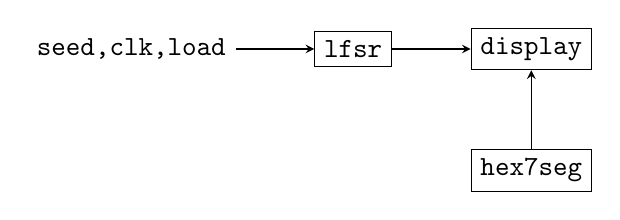
\begin{tikzpicture}[>=stealth]
        \node[draw] (lfsr) {\texttt{lfsr}};
        \node[draw, right=of lfsr] (display) {\texttt{display}};
        \node[draw, below=of display] (hex7seg) {\texttt{hex7seg}};
        \draw[->] (lfsr) -- (display);
        \draw[<-] (display) -- (hex7seg);
        \node[left=of lfsr] (in) {\texttt{seed,clk,load}};
        \draw[->] (in) -- (lfsr);
    \end{tikzpicture}
    \caption{顶层模块设计图}
    \label{fig:top}
\end{figure}

\section{实验总结与思考}

本次实验较为简单，基本是对在线评测的一个简单实机实现，没有遇到什么困难。

\section{思考题}

\textbf{生成的伪随机数序列仍然有一定的规律，如何能够生成更加复杂的伪随机数序列？}

可以考虑以下方式

\begin{enumerate}
    \item 增加寄存器的位数
    \item 选择更加复杂的组合逻辑
    \item 基于环境因素初始化种子
\end{enumerate}

\end{document}